\documentclass{standalone}
\usepackage{tikz}
\usepackage{pgfplots}
\pgfplotsset{compat=1.16}

\begin{document}
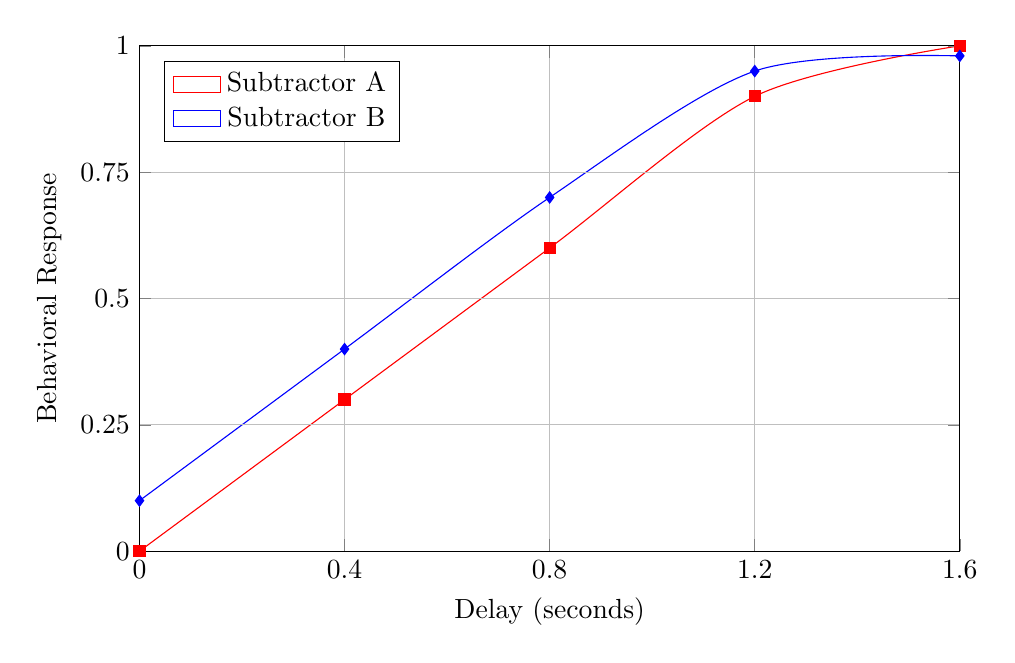
\begin{tikzpicture}
    \begin{axis}[
        width=12cm,
        height=8cm,
        xlabel={Delay (seconds)},
        ylabel={Behavioral Response},
        xmin=0,
        xmax=1.6,
        ymin=0,
        ymax=1,
        xtick={0,0.4,0.8,1.2,1.6},
        ytick={0,0.25,0.5,0.75,1},
        grid=major,
        legend pos=north west,
        area style,
        smooth
    ]
        
        % Red line for Subtractor A
        \addplot[red, mark=square*] coordinates {
            (0,0) (0.4,0.3) (0.8,0.6) (1.2,0.9) (1.6,1)
        };
        \label{subtractorA}
        
        % Blue line for Subtractor B
        \addplot[blue, mark=diamond*] coordinates {
            (0,0.1) (0.4,0.4) (0.8,0.7) (1.2,0.95) (1.6,0.98)
        };
        \label{subtractorB}
        
        % Legend
        \legend{Subtractor A, Subtractor B}
    \end{axis}
\end{tikzpicture}
\end{document}